\section{Messung der Oberflächenladung der Substrate mit dem Kelvin-Aufbau}

\subsection{Beschreibung des Aufbaus}
Die verwendete Kelvinsonde wurde im Rahmen der Diplomarbeit von \name{U. Moosbrugger} \cite{uli} aufgebaut und ist dort auch genauer beschrieben. Allerdings konnte die dort bestimmte Resonanzfrequenz von ca.\ \unit[390]{Hz} nicht reproduziert werden. Womöglich wurde der Aufbau -- hier speziell die schwingende Masse -- in der Zwischenzeit modifiziert.
\begin{figure}[h!tbp]
	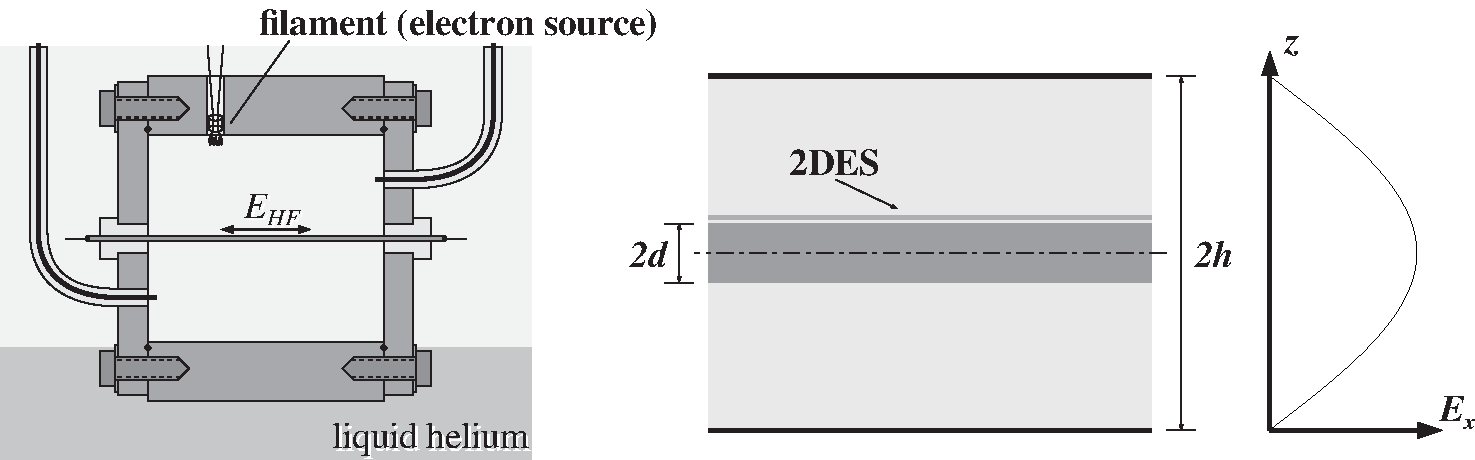
\includegraphics[width=\smidwidth]{exp_kelvin/schema}\hfill
	\begin{minipage}[b]{\textwidth-\tabcolsep-\smidwidth}
		\caption[Schema der Messung des Kelvinsignals]{Schema der Beschaltung der Elektroden des Kelvin-Aufbaus. Anstelle der Messung des Spannungsabfalls an einem Widerstand wurde ein LockIn-Verstärker EG\&G 5210 mit dem Strom-Spannungs-Wandler am Eingang verwendet.}
		\label{fig:kelvin_schema}
	\end{minipage}
\end{figure}

Gemessen wird im Folgenden der Strom, der durch das Bewegen des Sondenplättchens im äußeren elektrischen Feld influenziert wird.

\subsection{Messmethode der Kelvin"=Sonde}
\begin{figure}[h!tbp]
	\centerline{%
		\subfigure[ohne Probe]{\plotlink{spectrum_empty}{\includegraphics[width=\smallwidth]{exp_kelvin/spectrum_empty}}}%
		\subfigure[Silizium-Probe\label{fig:kelvin_si}]{\plotlink{spectrum}{\includegraphics[width=\smallwidth]{exp_kelvin/spectrum}}}}
	\caption[Resonanzkurven des Kelvin"=Aufbaus]{Vergleich der Resonanzen {\bfseries (a)} ohne Substrat und {\bfseries (b)} mit einem gereinigten und unbeladenem Silizium-Substrat bei verschiedenen Anregungsspannungen}
	\label{fig:kelvin_spectrum}
\end{figure}
In Abbildung~\ref{fig:kelvin_spectrum} sieht man mehrere Resonanzspektren des Kelvin-Aufbaus für den Fall der leeren Apparatur und für ein Silizium-Substrat unter der Sonde. Wie man sieht wird der Anteil von Nichtlinearitäten an der Resonanz ab einer Anregungsamplitude von \unit[750]{mV} bei beiden Messungen durch die zunehmende Asymmetrie der Resonanzlinie sehr deutlich. Deshalb wurden für alle folgenden Messungen deutlich geringere Amplituden gewählt. Der Unterschied in der Signalstärke bei der Messung ohne und mit Substrat ergibt sich aus der Tatsache, dass der Abstand der Sonde zur Substratunterlage bei allen Messungen konstant gehalten wurde. Für den Fall mit eingelegtem Substrat ist das elektrische Feld an der Sonde dann deutlich höher, da das Substrat als Dielektrikum wirkt.

\begin{figure}[h!tb]
	\centerline{%
		\subfigure[keine Probe]{\plotlink{xy_empty}{\includegraphics[width=\smallwidth]{exp_kelvin/xy_empty}}}%
		\subfigure[Silizium-Probe\label{fig:kelvin_ref_si}]{\plotlink{xy}{\includegraphics[width=\smallwidth]{exp_kelvin/xy}}}}
	\caption[Vergleich einer Kelvin"=Messung mit und ohne Substrat]{Messung des in der schwingenden Sonde influenzierten Stromes {\bfseries (a)} ohne und {\bfseries (b)} mit Substrat bei verschiedenen Frequenzen und verschiedenen Spannungen an der unteren Elektrode. Aufgetragen sind die Geraden der Spannungsdurchläufe von $-10$ bis $\unit[10]{V}$ der unteren Elektrode für verschiedene Frequenzen um die Resonanzfrequenz des Systems in der $xy$"=Darstellung vom $x$ gleich- und $y$ gegenphasigen Signal.}
	\label{fig:kelvin_ref}
\end{figure}Um die Beladung der Substratoberfläche zu untersuchen, wurde nun für verschiedene Frequenzen in der Nähe der oben bestimmten Resonanzfrequenz das Potential der unteren Elektrode von $-10$ bis \unit[10]{V} durchfahren und dabei der influenzierte Strom an der Sonde beobachtet. Die Ergebnisse dieser Messung am leeren Aufbau und mit einem unbeladenen Substrat sind in Abbildung~\ref{fig:kelvin_ref} zu sehen.
Mit dieser Methode ist es sehr einfach, die Änderung des elektrischen Feldes am Ort der Sonde in situ zu detektieren; dies ist auch die übliche Anwendung dieser Methode im Zusammenhang mit Messungen an Elektronen auf Helium \cite{Wil71,Etz84,Ara99}. Wenn man hingegen die Oberflächenladung auf verschiedenen Substraten bestimmen und vergleichen will, ist es sehr schwierig, quantitative Aussagen über die gemessenen Ergebnisse zu machen. Bei einem Wechsel des Substrats oder bei Bewegung der Sonde über das Substrat hinweg verändern sich die das Ausgangssignal bestimmenden Parameter, wie z.~B. der Abstand der Sonde zur Probe.
 
Der in der Sonde influenzierte Strom verschwindet nur dann, wenn das mittlere vertikale elektrische Feld an der Sonde verschwindet. 
\begin{figure}[h!tb]
	\begin{minipage}[b]{\smallwidth}%
	\plotlink{xy_charges}{\includegraphics[width=\smallwidth]{exp_kelvin/xy_charges}}%
	\end{minipage}
	\begin{minipage}[b]{\textwidth-\smallwidth-\tabcolsep}
		\caption[Influenzierter Sondenstrom bei Rampen der Spannung an der unteren Elektrode]{Influenzierter Sondenstrom bei Rampen der Spannung an der unteren Elektrode gemessen bei verschiedenen Frequenzen an einem beladenen PMMA/Silizium-Substrat \#69.\par
		Deutlich zu sehen ist die verstärkte Asymmetrie der Linien bezüglich ihres gemeinsamen Schnittpunkts, die auf das Vorhandensein von Ladung auf der Substratoberfläche hindeutet. Auftragung siehe Abbildung~\ref{fig:kelvin_ref}}
		\label{fig:kelvin_charges}
	\end{minipage}
\end{figure}
Dies passiert genau am Schnittpunkt aller Linien der Spannungsrampen in Abbildungen~\ref{fig:kelvin_ref} und \ref{fig:kelvin_charges}, der bei einem idealen Aufbau mit dem Ursprung der $xy$-Ebene zusammenfällt. Offensichtlich sorgt ein Anteil von kapazitivem Übersprechen am Signal dafür, dass dieser Schnittpunkt bei den hier gezeigten Ergebnissen etwas verschoben ist. Dieses Übersprechen wurde durch eine nicht optimale elektrische Trennung von Anregungskreis und Messelektrode verursacht, die durch Abschirmung der Zuleitungen verbessert werden konnte. Zusätzlich sieht man bei der unbeladenen Probe in Abbildung~\ref{fig:kelvin_ref_si} eine leichte Asymmetrie, die von den im System auftretenden Kontaktspannungen herrühren kann.
Den deutlichen Effekt von Oberflächenladungen sieht man in Abbildung~\ref{fig:kelvin_charges}, in der der Schnittpunkt der Geraden im Verleich zum unbeladenen Substrat deutlich verschoben ist.

\subsection{Auswertung der Messdaten}

Die Kelvin"=Methode zur Messung der Oberflächenladung wurde in der Literatur bisher \cite{Wil71,Etz84,Ara99,uli} sehr häufig verwendet, allerdings meist nur die Änderung des elektrischen Feldes infolge einer Änderung der Ladungsdichte in situ zu detektieren. Für den idealen Fall, dass die Gerade bei Durchlaufen der Spannung an der unteren Elektrode in der $xy$-Auftragung durch den Nullpunkt geht, ist die Amplitude des influenzierten Wechselstromes direkt proportional zum elektrischen Feld am Ort der Sonde. 

Schwieriger wird die Datenauswertung, wenn wie in diesem Fall die Beladung der Oberfläche von verschiedenen Substraten untersucht werden soll und auch absolute Werte der Beladung gewünscht sind. Nach Minimierung des kapazitiven Übersprechens kann man Spannungsrampen, die in der Nähe der Resonanzfrequenz aufgenommen wurden, auswerten. Über die Verschiebung der Projektion des Achsenursprungs auf die Gerade der Messpunkte kann man einen Hinweis auf die Ladung zwischen den beiden Elektroden erhalten.
